\documentclass[11pt]{article}

%----------%
% Packages %
%----------%

\usepackage{tikz}
\usepackage{fancyhdr}
\usepackage{enumitem}
\usepackage[letterpaper, margin=1in]{geometry}
\usepackage{upquote}
\usepackage[T1]{fontenc}
\usepackage{textcomp}
\usepackage{listings}
\usepackage{color}
\usepackage{inconsolata}
\usepackage{graphicx}
\usepackage{setspace}
\usepackage[most]{tcolorbox}
\usepackage{hyperref}
\usepackage{amssymb}

\usepackage{caption}
\captionsetup[lstlisting]{labelformat=empty,labelsep=none}

%-----------------%
% Header & footer %
%-----------------%

\pagestyle{fancy}
\lhead{Blobosle}
\rhead{CS 250}
\chead{Final (Notes)\\Spring 2025}
\cfoot{}
\rfoot{Page \thepage}

%-------%
% Title %
%-------%

\title{\textbf{CS 250: Computer Architecture\\Final Exam\\Spring 2025}}
\author{Benjamin Lobos Lertpunyaroj}
\date{\textit{May 8th, 10:30{\tiny AM} – 12:30{\tiny PM}}}

\setlength{\headsep}{3em}

%----------%
% Settings %
%----------%

\setlength{\parindent}{0pt}
\setstretch{1.5}

\definecolor{greenText}{rgb}{0.5, 0.7, 0.5}
\definecolor{greyText}{rgb}{0.5, 0.5, 0.5}
% \definecolor{codeFrame}{rgb}{0.5, 0.7, 0.5}
\definecolor{codeFrame}{rgb}{0.45, 0.66, 0.76}
\definecolor{moonstoneblue}{rgb}{0.45, 0.66, 0.76}
\definecolor{moondark}{rgb}{0.30, 0.50, 0.60}

\lstdefinestyle{code}{
  frame=single,
  rulecolor=\color{codeFrame},
  numbers=left,
  numbersep=8pt,
  numberstyle=\tiny\color{greyText},
  commentstyle=\color{greenText},
  basicstyle=\linespread{1.1}\ttfamily\footnotesize,
  keywordstyle=\ttfamily\footnotesize,
  showstringspaces=false,
  xleftmargin=1.95em,
  framexleftmargin=1.6em,
  breaklines=true,
  postbreak=\mbox{\textcolor{greenText}{$\hookrightarrow$}\space}
}
\lstset{style=code, language=C}

%------–-------%
% Initial page %
%--------------%

\begin{document}

\maketitle

\vspace{1em}

\begin{center}
\section*{Exam contents and details for referencing}
\end{center}

\begin{itemize}[itemsep=-0.5em, left=0pt, label={•}]
    \item Final exam is held in Fowler Hall on May 8th (Thursday), from 10:30 {\tiny AM} to 12:30 {\tiny PM}.
    \item Previous cumulative book chapters
    \vspace{-0.8em}
    \begin{itemize}[itemsep=-0.5em, left=0pt, label={•}]
    \item Chapter 1 sections 1, 2, and 3.
    \item Chapter 2, sections 1, 2, 3, 4, 5, 6, and 7.
    \item Chapter 3, sections 1, 2, and 5.
    \item Chapter 4, sections 1, 2, 3, 4, 5, 6, 7, and 8.
    \item Chapter 5, sections 1, 2, 3, 4, 7, and 8.
    \item Chapter 8 (Appendix A), sections 1, 2, 3 (but not PLAs or ROMs), 5, 7 (lightly), and 8.
    \end{itemize}
    \item All lecture notes and lecture slides.
    \item All labs (1 - 11).
\end{itemize}

\pagebreak

\section*{Appendix A}

\subsection*{Logic \& Gates}
An \textit{asserted} signal is logically true, the \textit{deasserted} is the opposite.

\begin{tcolorbox}[
    enhanced,
    attach boxed title to top left={xshift=6mm,yshift=-1.5mm},
    colback=moonstoneblue!20,
    colframe=moonstoneblue,
    colbacktitle=moonstoneblue,
    title=Two types of logic systems,
    fonttitle=\bfseries\color{white},
    boxed title style={size=small,colframe=moonstoneblue,sharp corners},
    sharp corners,
    label=box:logic-types,
]
    {\color{moondark}\textbf{Combinational logic}}: No memory in components, hence same output given same input. \\
    {\color{moondark}\textbf{Sequential logic}}: Memory in components, hence output depends on input and current memory state.
\end{tcolorbox}

\begin{figure}[htbp]
    \centering
    \fcolorbox{codeFrame}{white}{
        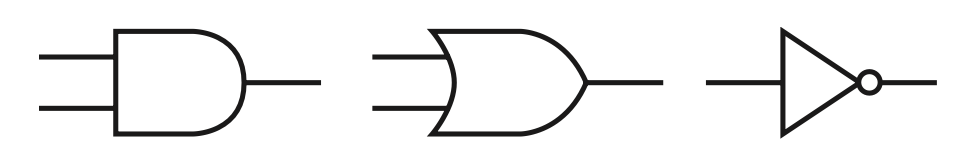
\includegraphics[width=0.5\linewidth]{img/gates.png}%
    }
    \caption{\textit{\texttt{AND} gate, \texttt{OR} gate, and inverter}}
\end{figure}

The gates can be combined to form different forms of logic. An example of this is $\overline{\overline{A} + B}$ which is equivalent to $A \cdot \overline{B}$ by De Morgan's law, seen in \autoref{fig:gates2}.

\begin{figure}[htbp]
    \centering
    \fcolorbox{codeFrame}{white}{
        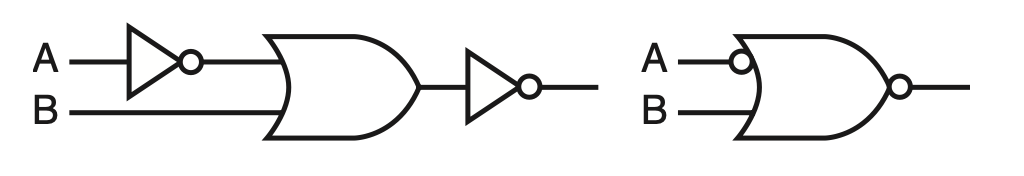
\includegraphics[width=0.5\linewidth]{img/gates2.png}%
    }
    \caption{\textit{Logic gate implementation of example formula}}
    \label{fig:gates2}
\end{figure}

\subsection*{Decoders \& Multiplexors}

A \textbf{decoder} is a logic block that has an n-bit input and $2^n$ outputs, where there is one unique true bit as output from a unique set of bytes of input.

\begin{figure}[htbp]
    \centering
    \fcolorbox{codeFrame}{white}{
        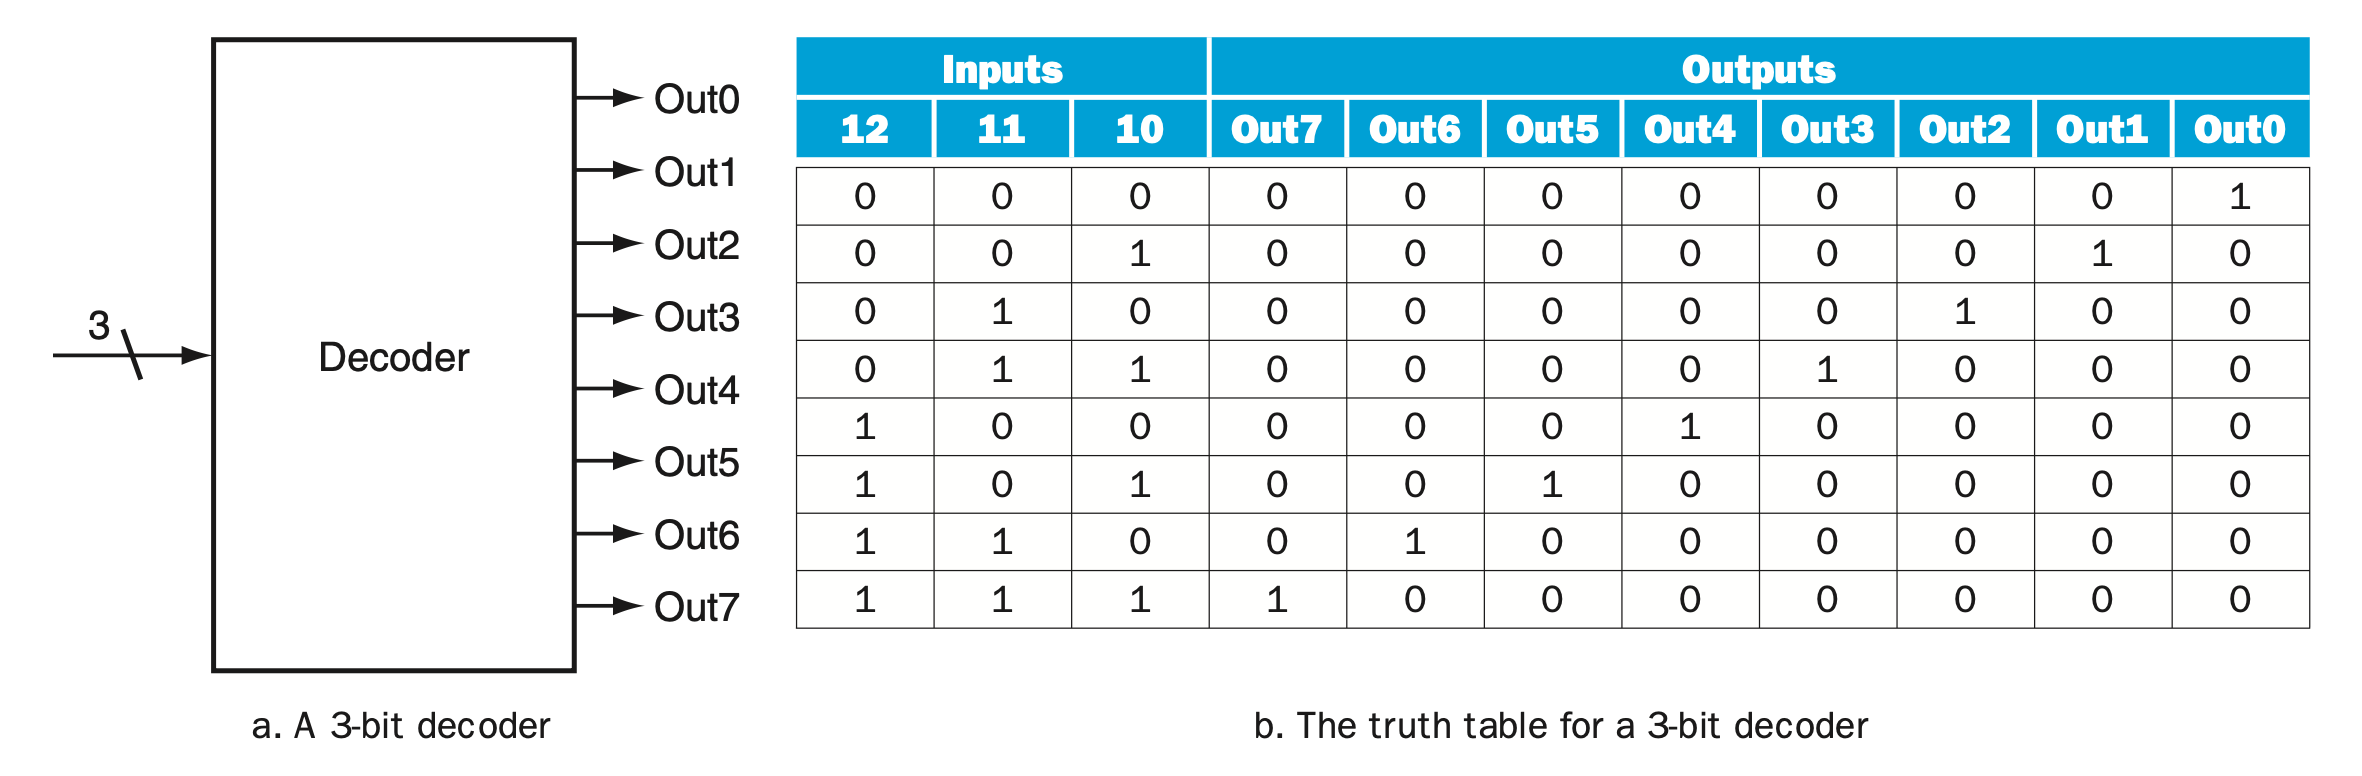
\includegraphics[width=0.7\linewidth]{img/decoder1.png}
    }
    \caption{\textit{3-bit input decoder that generates $2^3=8$ different outputs (Out0 – Out7)}}
\end{figure}

$$2^n \text{ outputs} \ \therefore \ \log_2{(\text{output})} = \text{input bits}$$

Encoders are the other way around.

\textbf{Multiplexors} have a selector input (or control value), that will determine which inputs will become outputs.

In the case of the two-input MUX, its representation is the following, $C=(A \cdot \overline{S}) +(B \cdot S)$, using n (data inputs) AND gates, and one OR gate.

\begin{figure}[htbp]
    \centering
    \fcolorbox{codeFrame}{white}{
        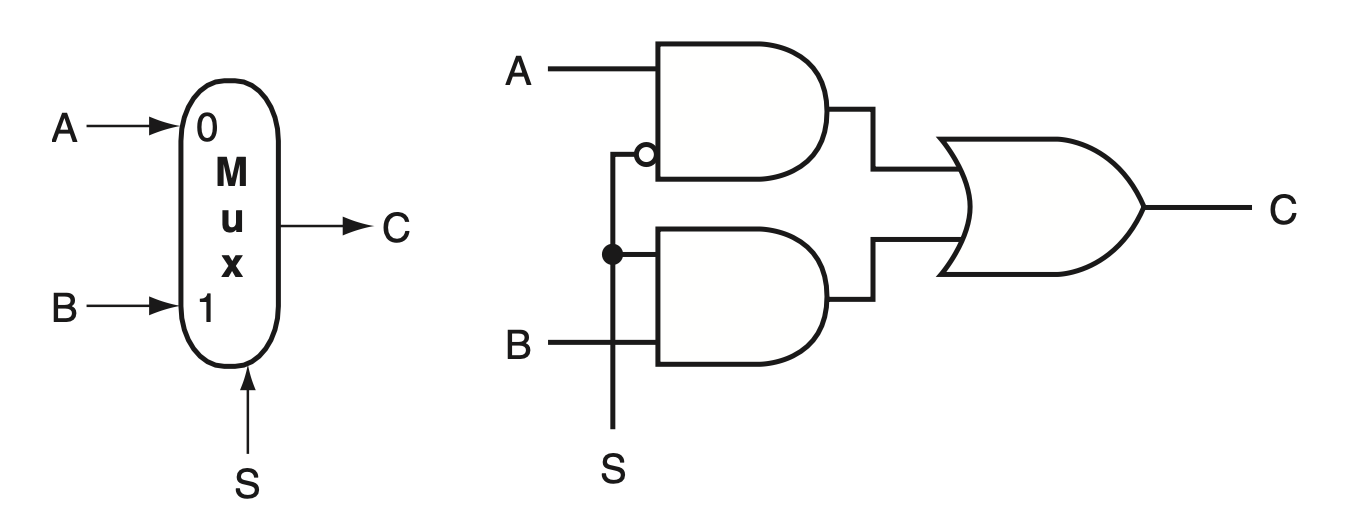
\includegraphics[width=0.5\linewidth]{img/mux1.png}
    }
    \caption{\textit{Two-input multiplexor that generates one output depending on the selector input S}}
\end{figure}

\vspace{-2.5em}
$$n \text{ (data inputs)} \therefore \log_2{n} = S \text{ selector bits required to represent all inputs}$$

Often times a decoder generates n bits for a MUX, to be used as a selector signal.

\subsection*{Buses}

A collection of data lines that is treated as a single logical signal.

When showing a logic unit whose inputs and outputs are buses, the unit must be replicated a sufficient number of times to accommodate the width of the input.

You can use multiplexors to select between two buses, requiring n inputs to represent n-bit buses.

\begin{figure}[htbp]
    \centering
    \fcolorbox{codeFrame}{white}{
        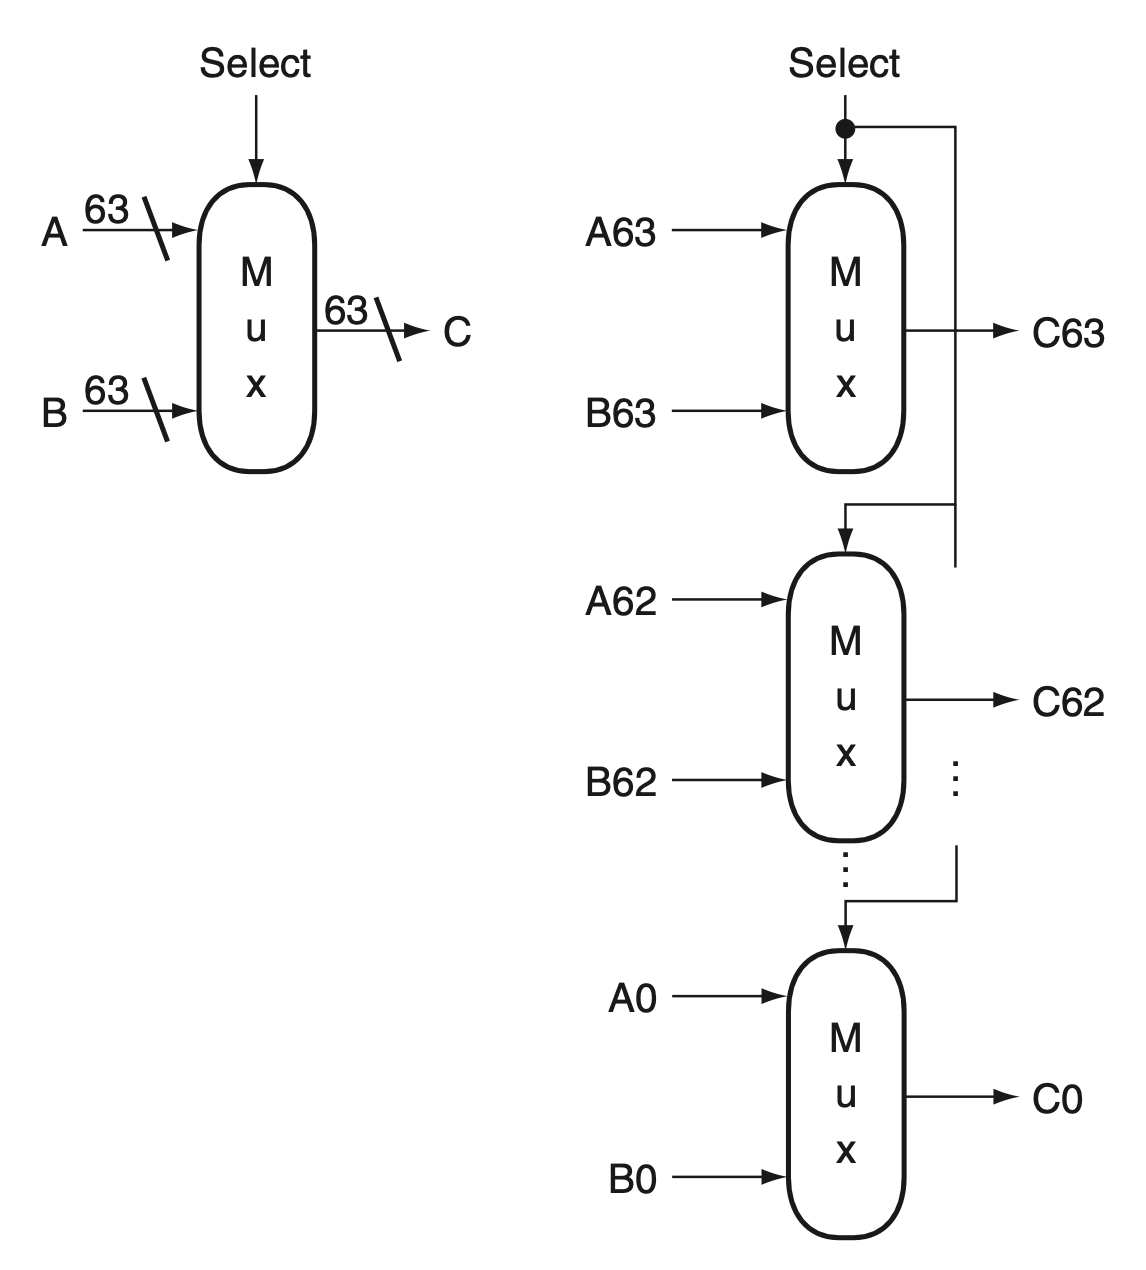
\includegraphics[width=0.28\linewidth]{img/bus1.png}
    }
    \caption{\textit{1-bit multiplexors replicated 64 times to represent two 64-bit buses}}
\end{figure}

\subsection*{ALUs}

\begin{tcolorbox}[
    enhanced,
    attach boxed title to top left={xshift=6mm,yshift=-1.5mm},
    colback=moonstoneblue!20,
    colframe=moonstoneblue,
    colbacktitle=moonstoneblue,
    title=Operation done by the ALU,
    fonttitle=\bfseries\color{white},
    boxed title style={size=small,colframe=moonstoneblue,sharp corners},
    sharp corners,
]
    {\color{moondark}\textbf{Logic operations}}: \texttt{AND} and \texttt{OR} gate operations, with \texttt{NOR} being available through an inversion of both input signals with \texttt{AInvert} and \texttt{BInvert} control signals. \\
    {\color{moondark}\textbf{Arithmetic operations}}: Addition and subtraction through the full adder, and \texttt{BInvert} control signal on one input for determining the type of operation.
\end{tcolorbox}

The LEGv8 word is 64 bits wide, as such a 64 bit wide ALU is required (64 1-bit ALUs).

In its simplest form, a \underline{1-bit logical unit} for \texttt{AND} and \texttt{OR} operations simply requires a multiplexor an a one bit control signal to select between the two operations ($2^1=1$).

\begin{figure}[htbp]
    \centering
    \fcolorbox{codeFrame}{white}{
        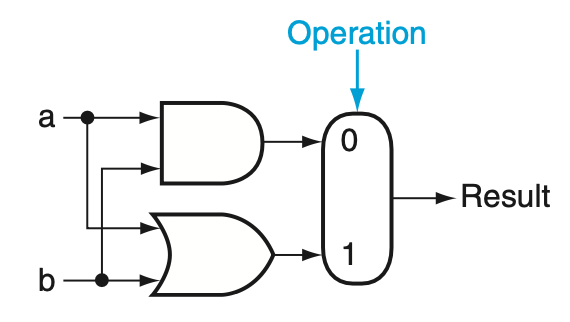
\includegraphics[width=0.28\linewidth]{img/alu1.png}
    }
    \caption{\textit{1-bit logical unit for \texttt{AND} and \texttt{OR} operations}}
\end{figure}

Implementing addition requires two input operands, one output, a \texttt{CarryIn} bit carried from the less-significant bits of the operation (i.e. another 1-bit logical unit), and a \texttt{CarryOut} bit to be carried forward to the next more significant bit.

\begin{figure}[htbp]
    \centering
    \fcolorbox{codeFrame}{white}{
        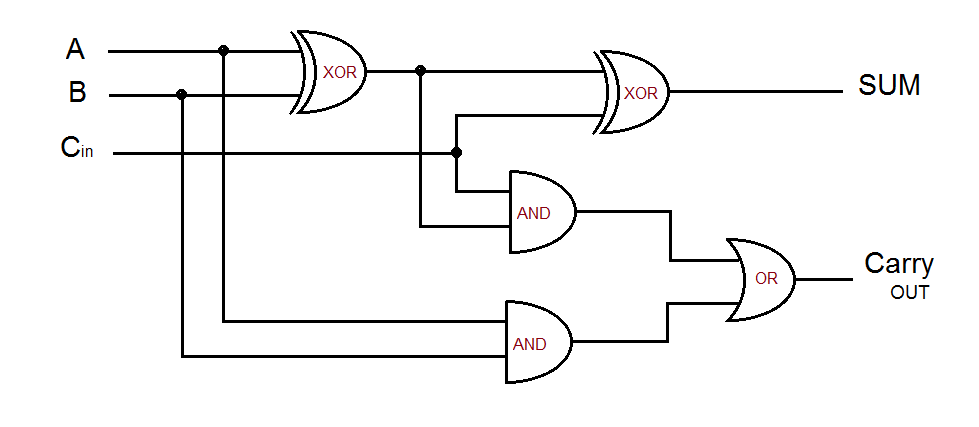
\includegraphics[width=0.8\linewidth]{img/adder1.png}
    }
    \caption{\textit{Full adder that performs mod 2 addition}}
\end{figure}

The combination of the adder and the logic gates, coupled with a multiplexor with a control signal to determine the operation makes a complete 1-bit ALU, which can be seen in \autoref{fig:1bitalu}.
\pagebreak

\begin{figure}[htbp]
    \centering
    \fcolorbox{codeFrame}{white}{
        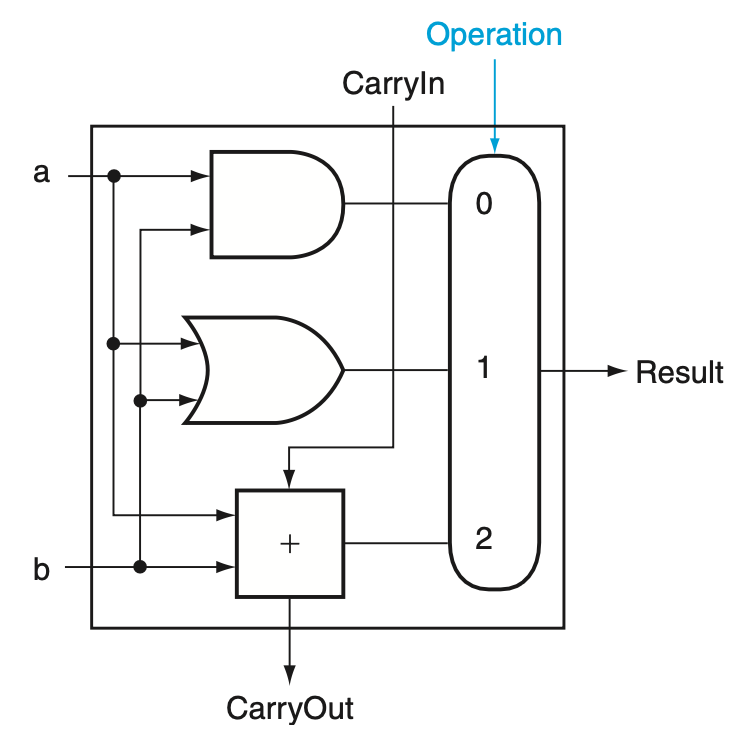
\includegraphics[width=0.2\linewidth]{img/alu2.png}
    }
    \caption{\textit{1-bit alu with logical operations and addition}}
    \label{fig:1bitalu}
\end{figure}

For expanding to a 64-bit ALU, the adders have to set up a ripple carry from the least to the most significant bit.

\begin{figure}[htbp]
    \centering
    \fcolorbox{codeFrame}{white}{
        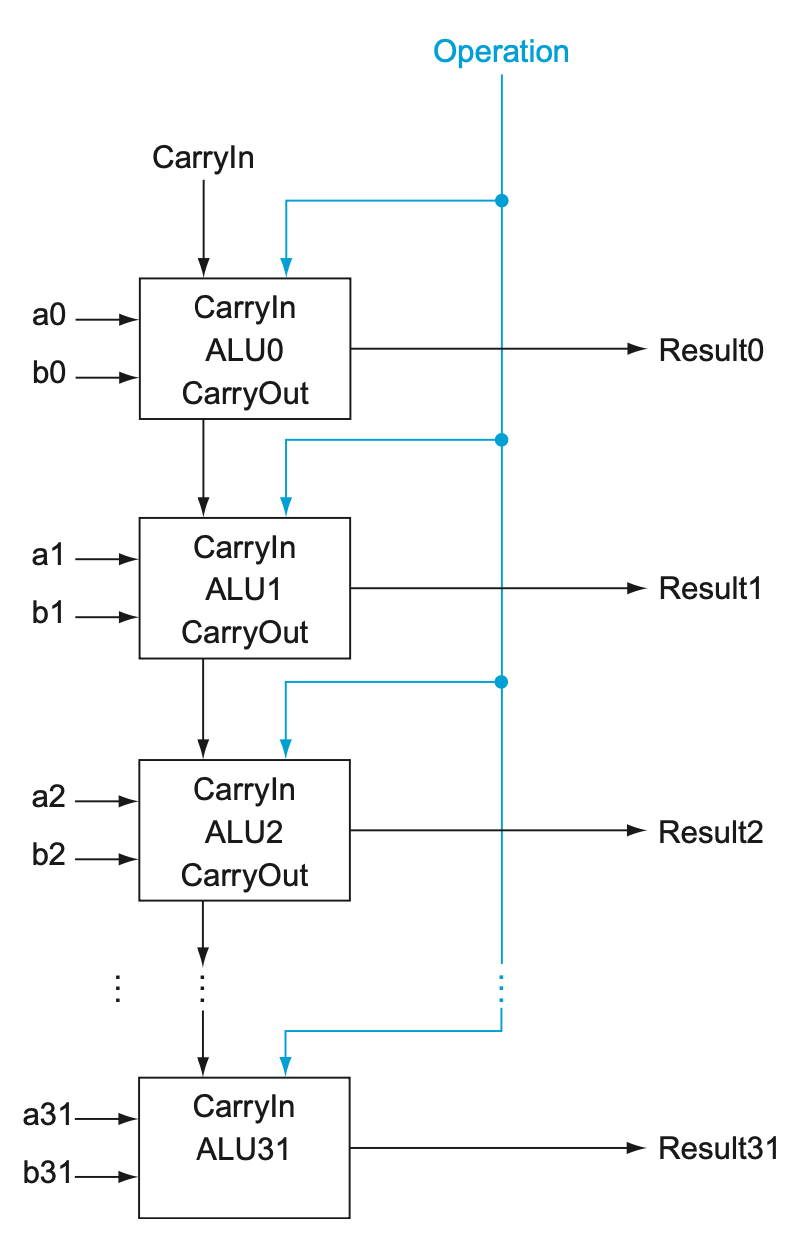
\includegraphics[width=0.2\linewidth]{img/ripplecarry.png}
    }
    \caption{\textit{Ripple carry implemented for a 64-bit ALU}}
\end{figure}

By inverting the second input (\texttt{BInvert} = 1, seen in \autoref{fig:subalu}) and setting \texttt{CarryIn} to 1 in the least significant bit of the ALU, we get two’s complement subtraction of \texttt{b} from \texttt{a}.

To implement a \texttt{NOR} function, existing components can be combined, $(\overline{a+b})=\overline{a} \cdot \overline{b}$ (DeMorgan's theorem), which means we need an \texttt{AND} and two inverters for both \texttt{a} and \texttt{b}, seen in \autoref{fig:subalu}

\begin{figure}[htbp]
    \centering
    \fcolorbox{codeFrame}{white}{
        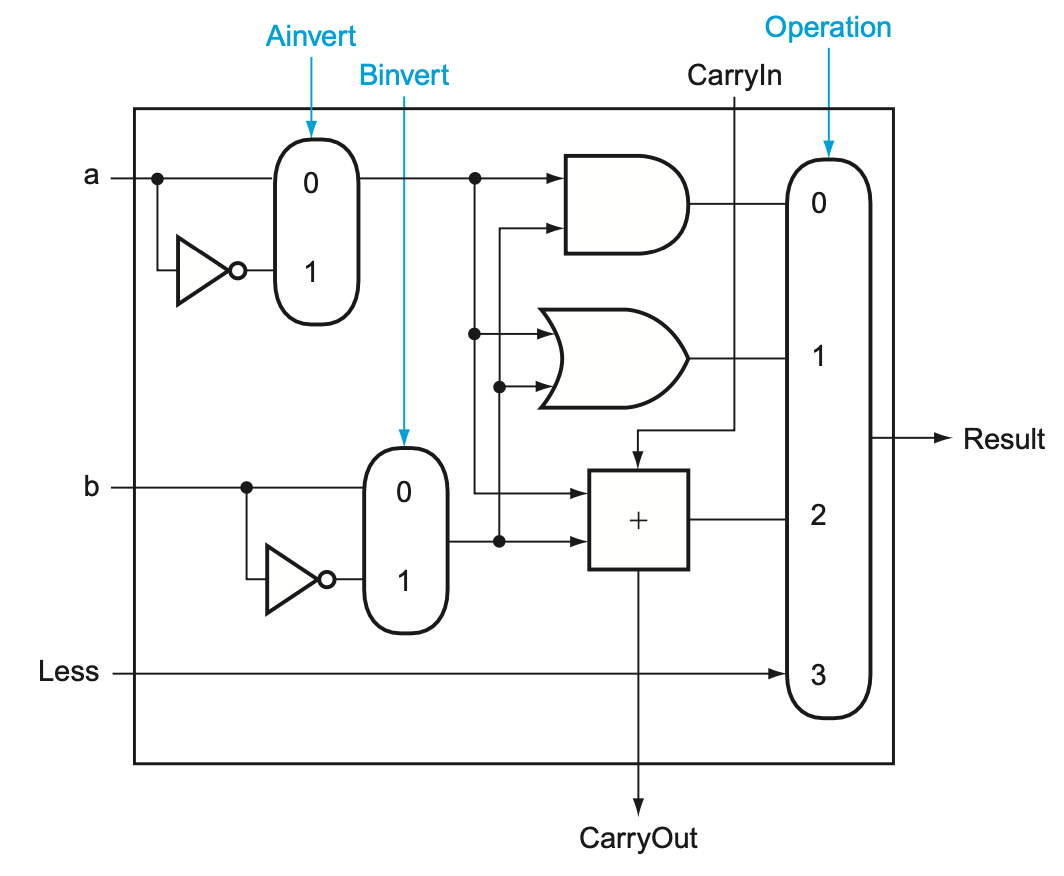
\includegraphics[width=0.32\linewidth]{img/alu3.png}
    }
    \caption{\textit{1-bit ALU that performs subtraction, and \texttt{NOR} operations}}
    \label{fig:subalu}
\end{figure}

On a 64-bit ALU we can use a zero flag to help with conditional branch instructions in LEGv8 (e.g. \texttt{CBZ}), as they receive to inputs and require to test if the subtraction has a zero.

The following represents this with an inversion of an \texttt{OR} tree on all results from the subtraction considering a 64-bit subtraction, fully represented in \autoref{fig:64aluzero}.
\vspace{-1em}
$$Zero = \overline{(R_0 + R_1 + R_2 + ... + R_{63})}$$
\vspace{-3em}

\begin{figure}[htbp]
    \centering
    \fcolorbox{codeFrame}{white}{
       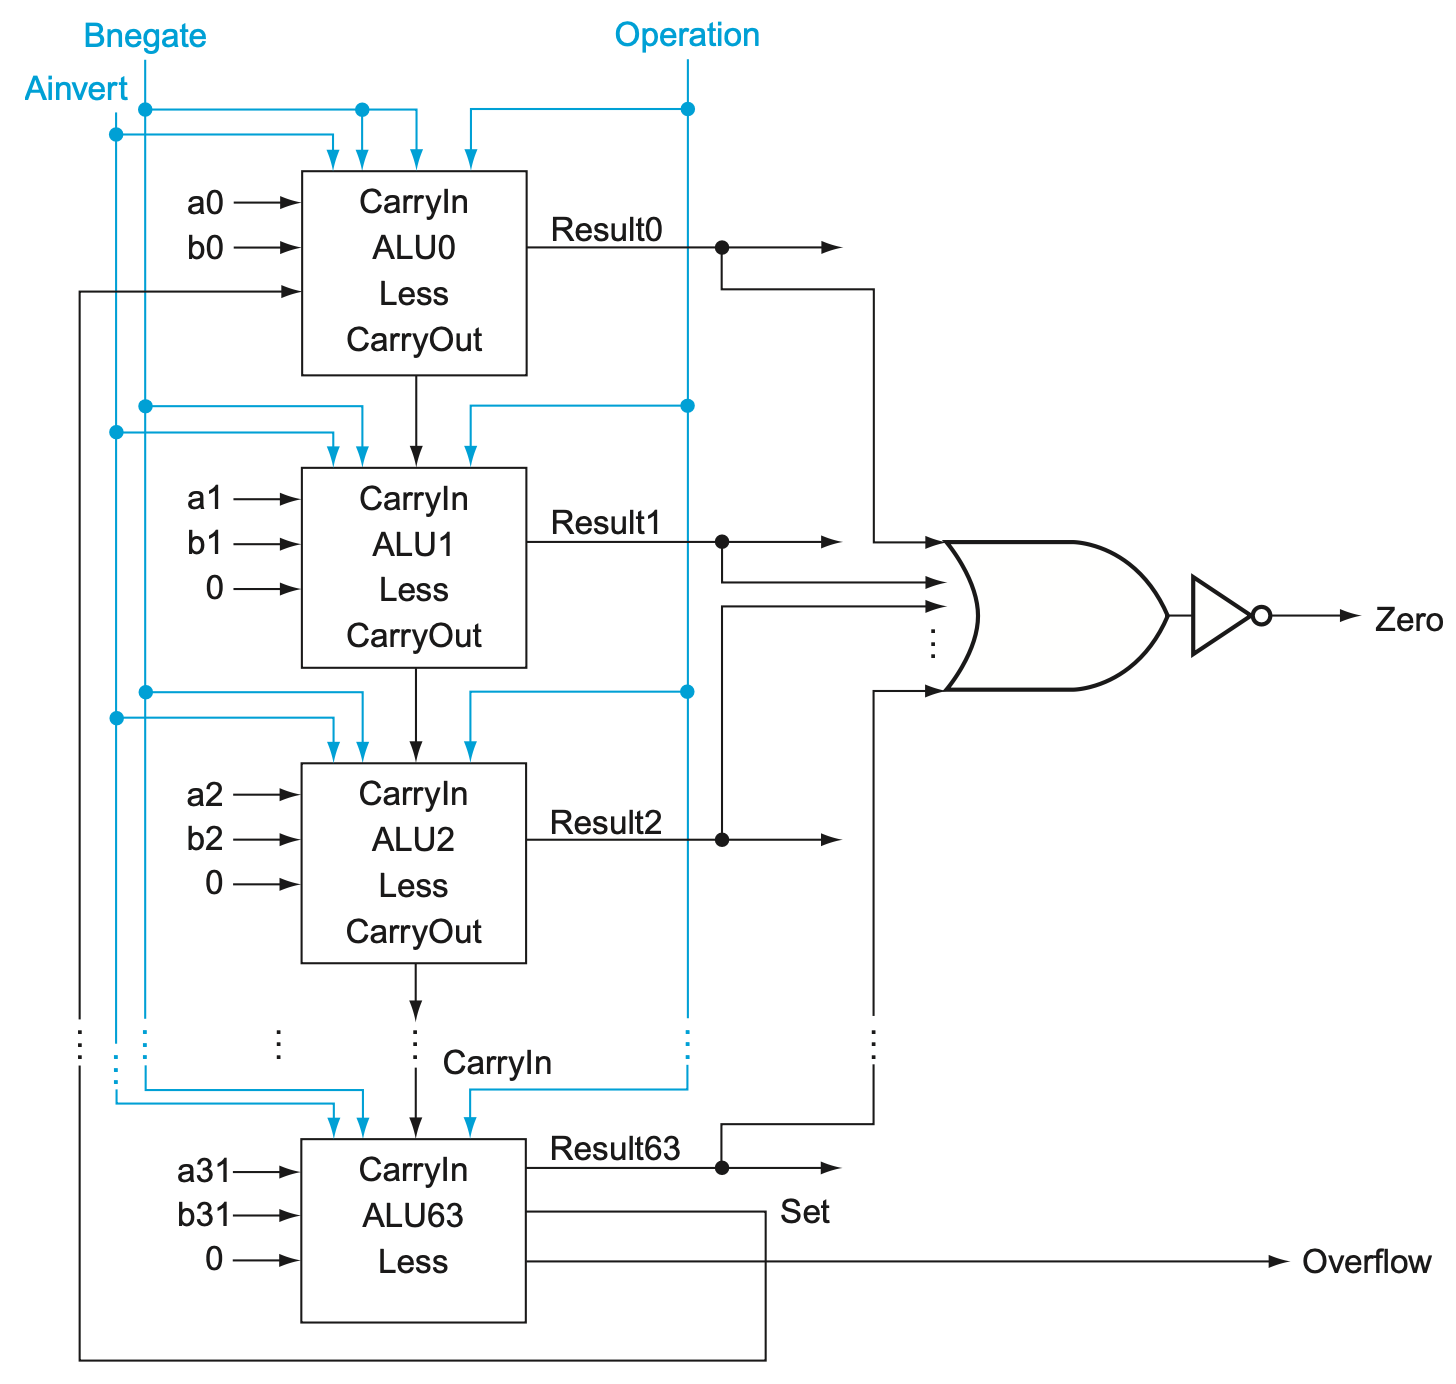
\includegraphics[width=0.4\linewidth]{img/alu4.png}
    }
    \caption{\textit{64-bit ALU \texttt{OR} tree and an inverter for determining the Zero flag}}
    \label{fig:64aluzero}
\end{figure}

For a generalized symbol of the ALU, \autoref{fig:generalalu}, where \texttt{ALU operation} is the control signal of the MUX that determines the type of operation.

\begin{figure}[htbp]
    \centering
    \fcolorbox{codeFrame}{white}{
       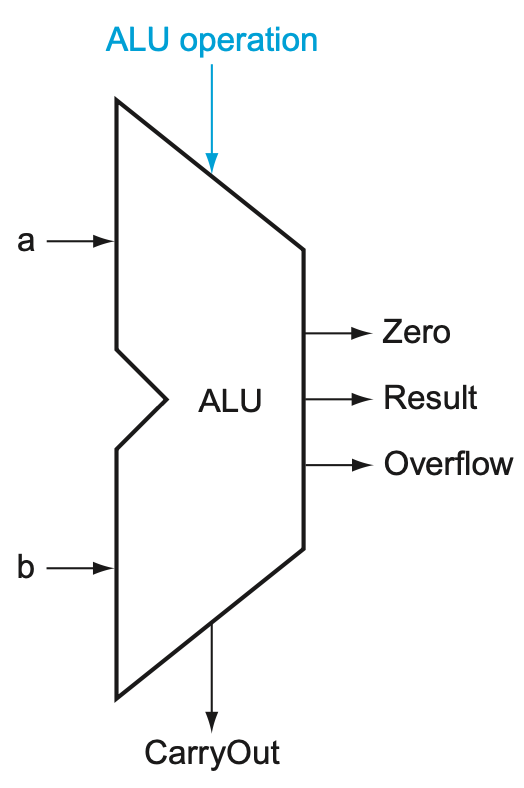
\includegraphics[width=0.2\linewidth]{img/alu5.png}
    }
    \caption{\textit{General symbol for an ALU or an adder}}
    \label{fig:generalalu}
\end{figure}

\pagebreak

\subsection*{Clocks}

\begin{tcolorbox}[
    enhanced,
    attach boxed title to top left={xshift=6mm,yshift=-1.5mm},
    colback=moonstoneblue!20,
    colframe=moonstoneblue,
    colbacktitle=moonstoneblue,
    title=Clocking methodology semantics,
    fonttitle=\bfseries\color{white},
    boxed title style={size=small,colframe=moonstoneblue,sharp corners},
    sharp corners,
]
    {\color{moondark}\textbf{Edge triggered clocking}}: State changes occur on a clock edge. \\
    {\color{moondark}\textbf{Synchronous system}}: Type of memory system where data is read only when a clock signal indicates stability (i.e. non-changing value).
\end{tcolorbox}

A \hyperref[box:logic-types]{combinational logic block}, recieves an input and then generates an output for a state element which is updated on a clock edge.

An edge-triggered methodology allows a state element to be read and written in the same clock cycle without creating a race condition.

For this to work, the clock cycle must be long enough for the state element to have received a stable input before the next active clock edge.

\begin{figure}[htbp]
    \centering
    \fcolorbox{codeFrame}{white}{
       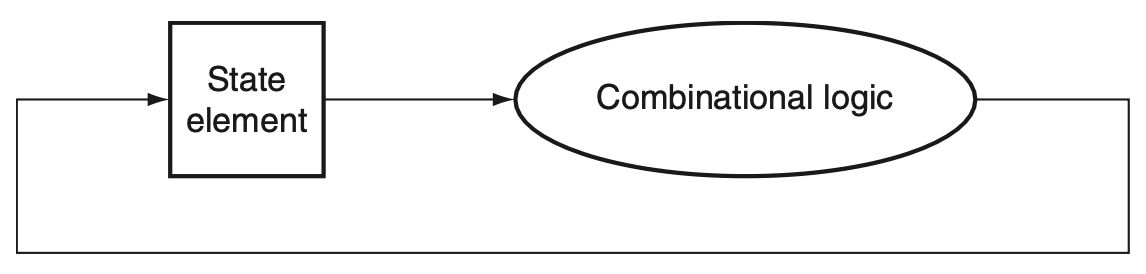
\includegraphics[width=0.5\linewidth]{img/clock1.png}
    }
    \caption{\textit{Edge-triggered state element to be read and written to in one active clock edge}}
\end{figure}

One such state element is the register file.

\subsection*{Flip-flops \& Latches}

\begin{tcolorbox}[
    enhanced,
    attach boxed title to top left={xshift=6mm,yshift=-1.5mm},
    colback=moonstoneblue!20,
    colframe=moonstoneblue,
    colbacktitle=moonstoneblue,
    title=Types of clocked memory elements,
    fonttitle=\bfseries\color{white},
    boxed title style={size=small,colframe=moonstoneblue,sharp corners},
    sharp corners,
]
    {\color{moondark}\textbf{Flip-flops}}: Edge-triggered element that changes the stored state only at a clock edge. \\
    {\color{moondark}\textbf{Latches}}: Level-sensitive element that changes the stored state at any time the clock is asserted.
\end{tcolorbox}

Flip-flops are build upon latches and are going to be used in edge-triggered systems.

A \textbf{D flip-flop} or \textbf{D latch} is used for storing the value of one data input signal, in the internal memory, at the clock edge.

To implement a \textbf{D latch}, it requires two inputs, the data to be stored \texttt{D}, and the clock signal \texttt{C}, producing two outputs, the value of the internal state \texttt{Q}, and its complement \(\overline{\mathtt{Q}}\).

The \hyperref[]{implementation} has cross-coupled \texttt{NOR} gates that store the state value unless \texttt{C} is asserted, in which case \texttt{D} replaces the value of \texttt{Q} and is stored.

\pagebreak

\begin{figure}[htbp]
    \centering
    \fcolorbox{codeFrame}{white}{
       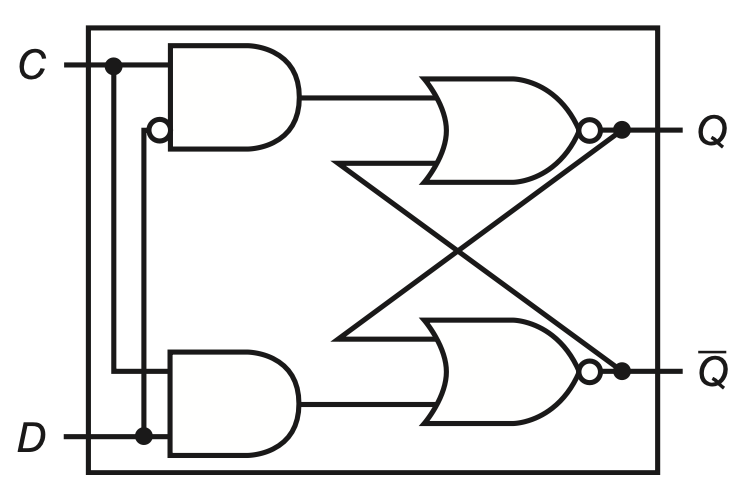
\includegraphics[width=0.3\linewidth]{img/dlatch.png}
    }
    \caption{\textit{D latch, composed of crossed \texttt{NOR} gates and a \texttt{SR} latch}}
    \vspace{1em}
    \centering
    \fcolorbox{codeFrame}{white}{
       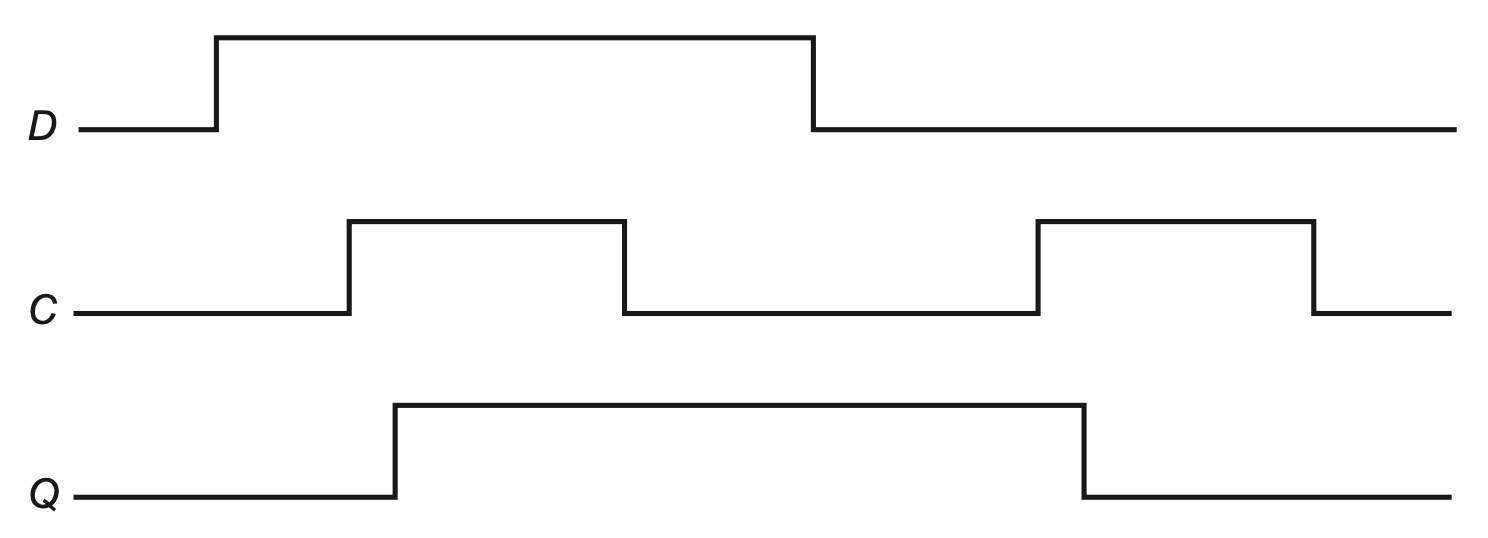
\includegraphics[width=0.35\linewidth]{img/dlatch1.png}
    }
    \caption{\textit{Progression of a D latch, assuming output is initially deasserted}}
\end{figure}

To implement a \textbf{D flip-flop}, with a \underline{falling-edge trigger}, we can use two D latches, master and slave. Master sets input \texttt{D} when \texttt{C} is asserted. When \texttt{C} falls, master is closed, but slave is open and gets its input from master's \texttt{Q}.

In this sense, the rising-edge represents when the master takes in the \texttt{D} value, and the falling-edge represents when the slave takes in the master's \texttt{D} producing the final \texttt{Q}.

\begin{figure}[htbp]
    \centering
    \fcolorbox{codeFrame}{white}{
       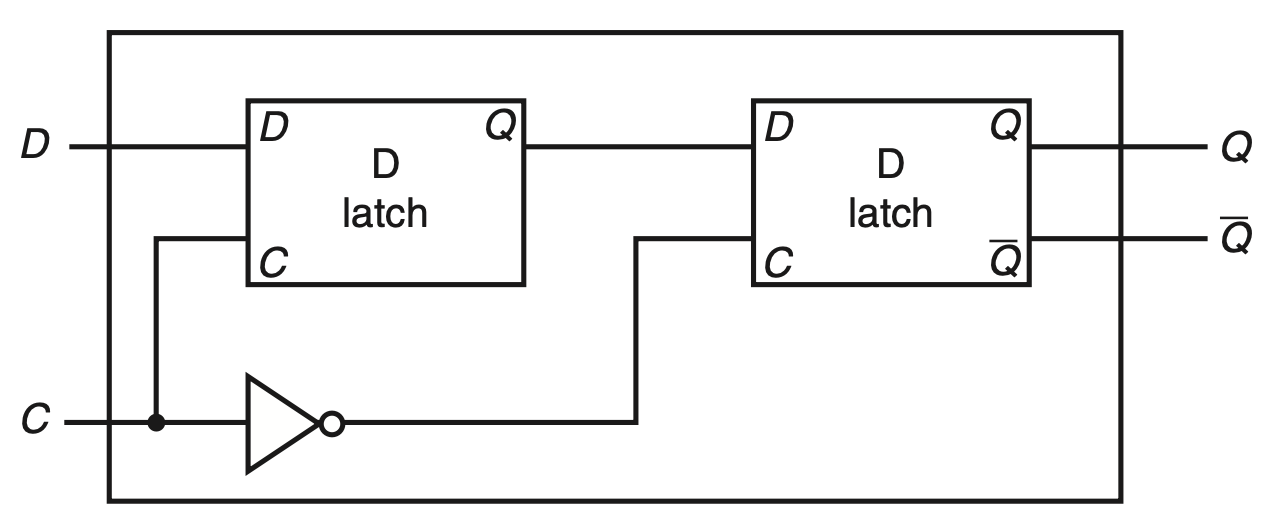
\includegraphics[width=0.5\linewidth]{img/dflip.png}
    }
    \caption{\textit{D flip-flop with a falling-edge trigger made from two D latches, master and slave}}
    \vspace{1.5em}
    \centering
    \fcolorbox{codeFrame}{white}{
       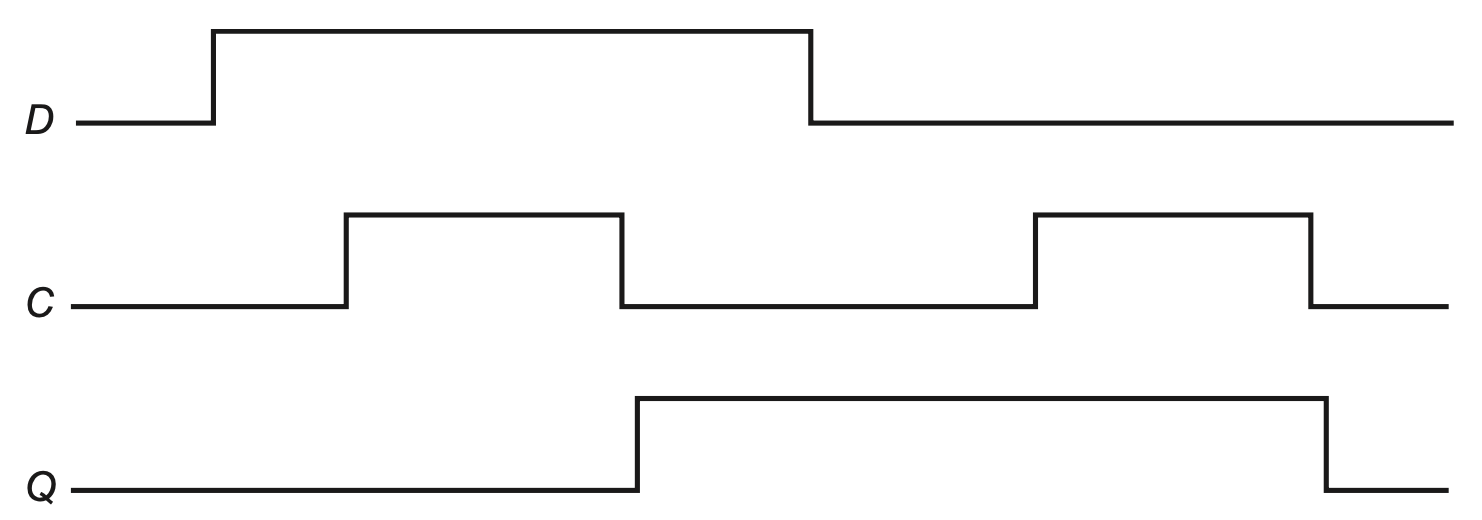
\includegraphics[width=0.5\linewidth]{img/dflip1.png}
    }
    \caption{\textit{Progression of a D flip-flop with a falling-edge trigger, where output is initially deasserted}}
\end{figure}

The minimum time \texttt{D} must retain a valid input is the setup time plus the hold time (after edge).

\subsection*{Register files}

A \textbf{register file} consists of a bunch of \textbf{registers} that can be read and written to, and a \texttt{WriteReg} control signal (clock).

For writing it requires the control signal, the number of the register to write to (\texttt{Write register}), and the data to write (\texttt{Write data}).

For reading it requires the numbers of the registers to read from (\texttt{Read register number 1 \& 2}), and it outputs the read contents from two registers (\texttt{Read data 1 \& 2}).

\begin{figure}[htbp]
    \centering
    \fcolorbox{codeFrame}{white}{
       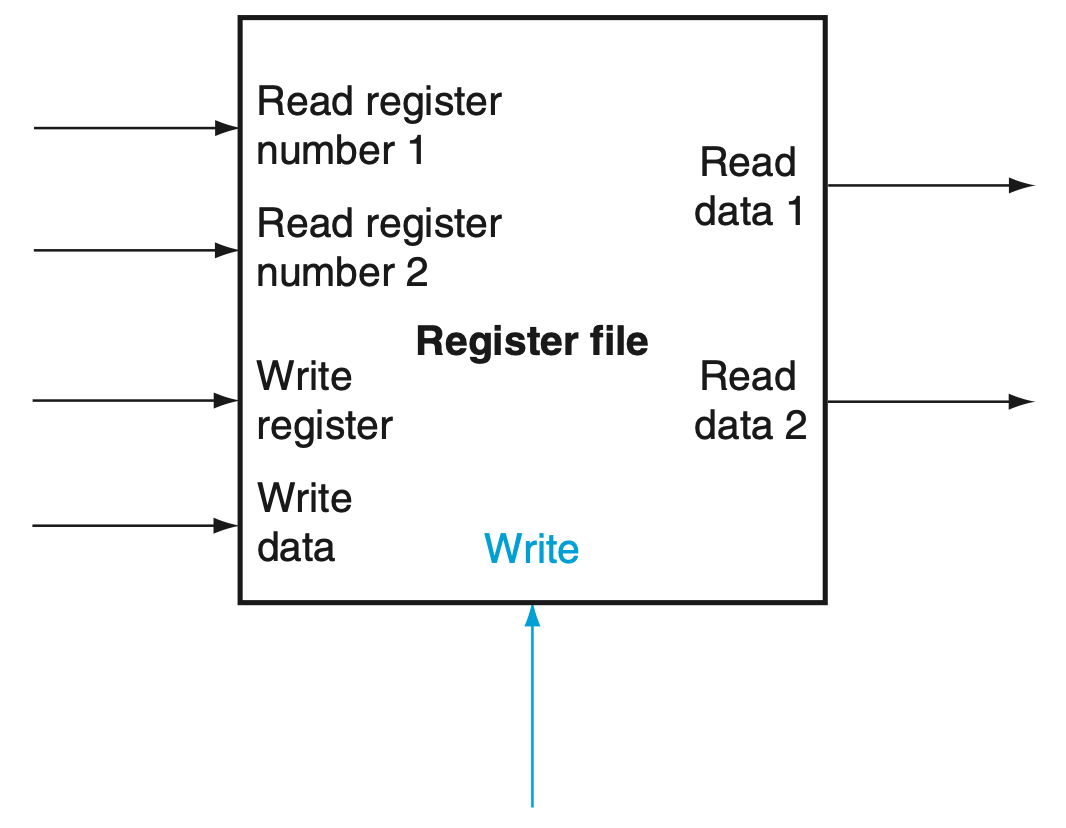
\includegraphics[width=0.35\linewidth]{img/regfile1.png}
    }
    \caption{\textit{Register file with two read ports and one write port}}
\end{figure}

The implementation for the \underline{write port} consists of a decoder that will select one of the \texttt{n - 1} registers that will be \texttt{AND}ed with the \texttt{WriteReg} signal to act as the \texttt{C} input for the registers (D flip-flops). The \texttt{D} input for every register is the \texttt{Write data} input from the reg. file.

\begin{figure}[htbp]
    \centering
    \fcolorbox{codeFrame}{white}{
       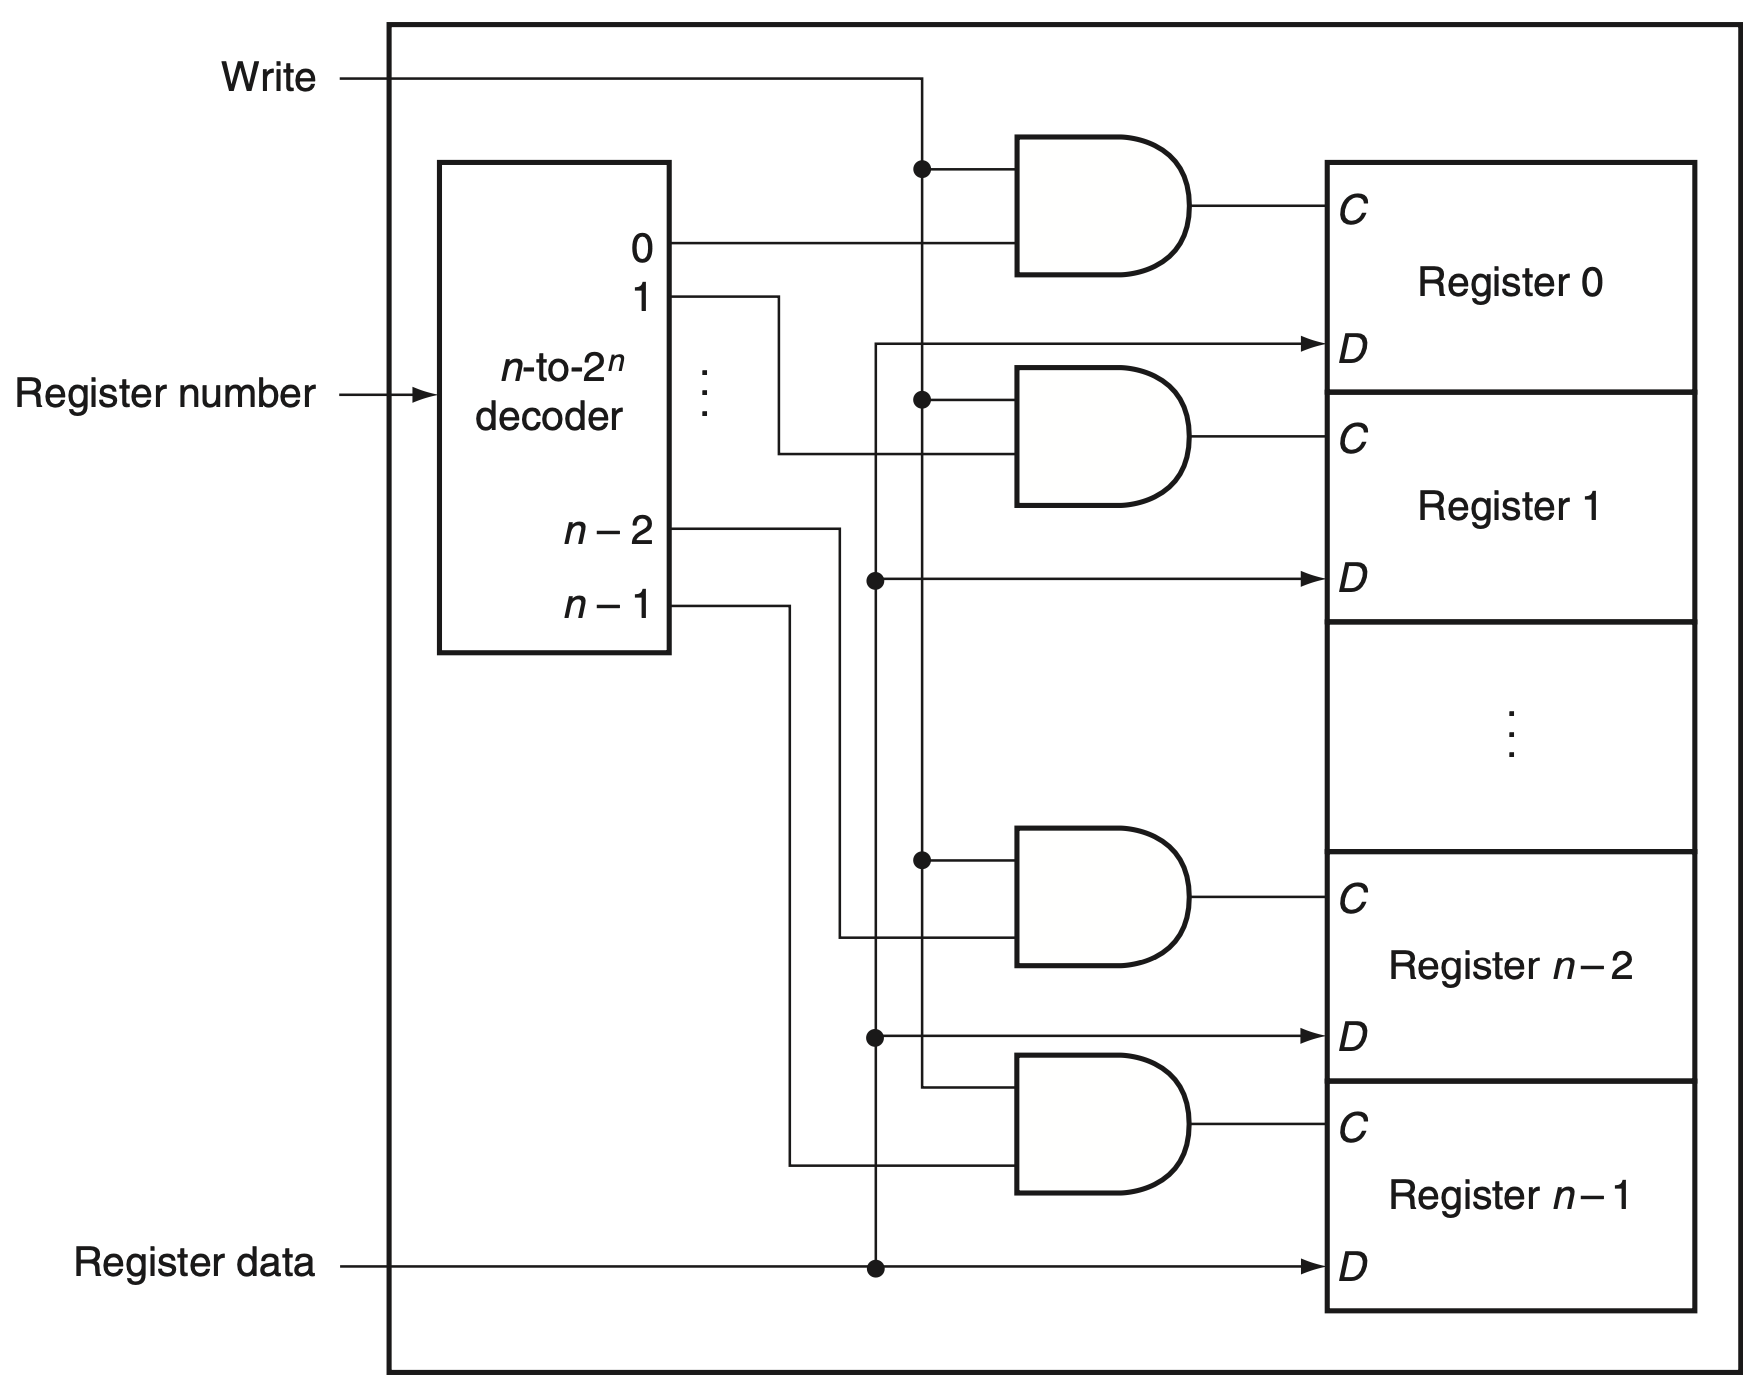
\includegraphics[width=0.55\linewidth]{img/regwrite1.png}
    }
    \caption{\textit{Write implementation in the register file}}
\end{figure}

The implementation for the two \underline{read ports} consists of using the stored state of the registers (\texttt{Q} output), as inputs for two different MUXes that use the \texttt{Read register number 1 \& 2} reg. file inputs as control signals to output the information of the two registers specified.

\begin{figure}[htbp]
    \centering
    \fcolorbox{codeFrame}{white}{
       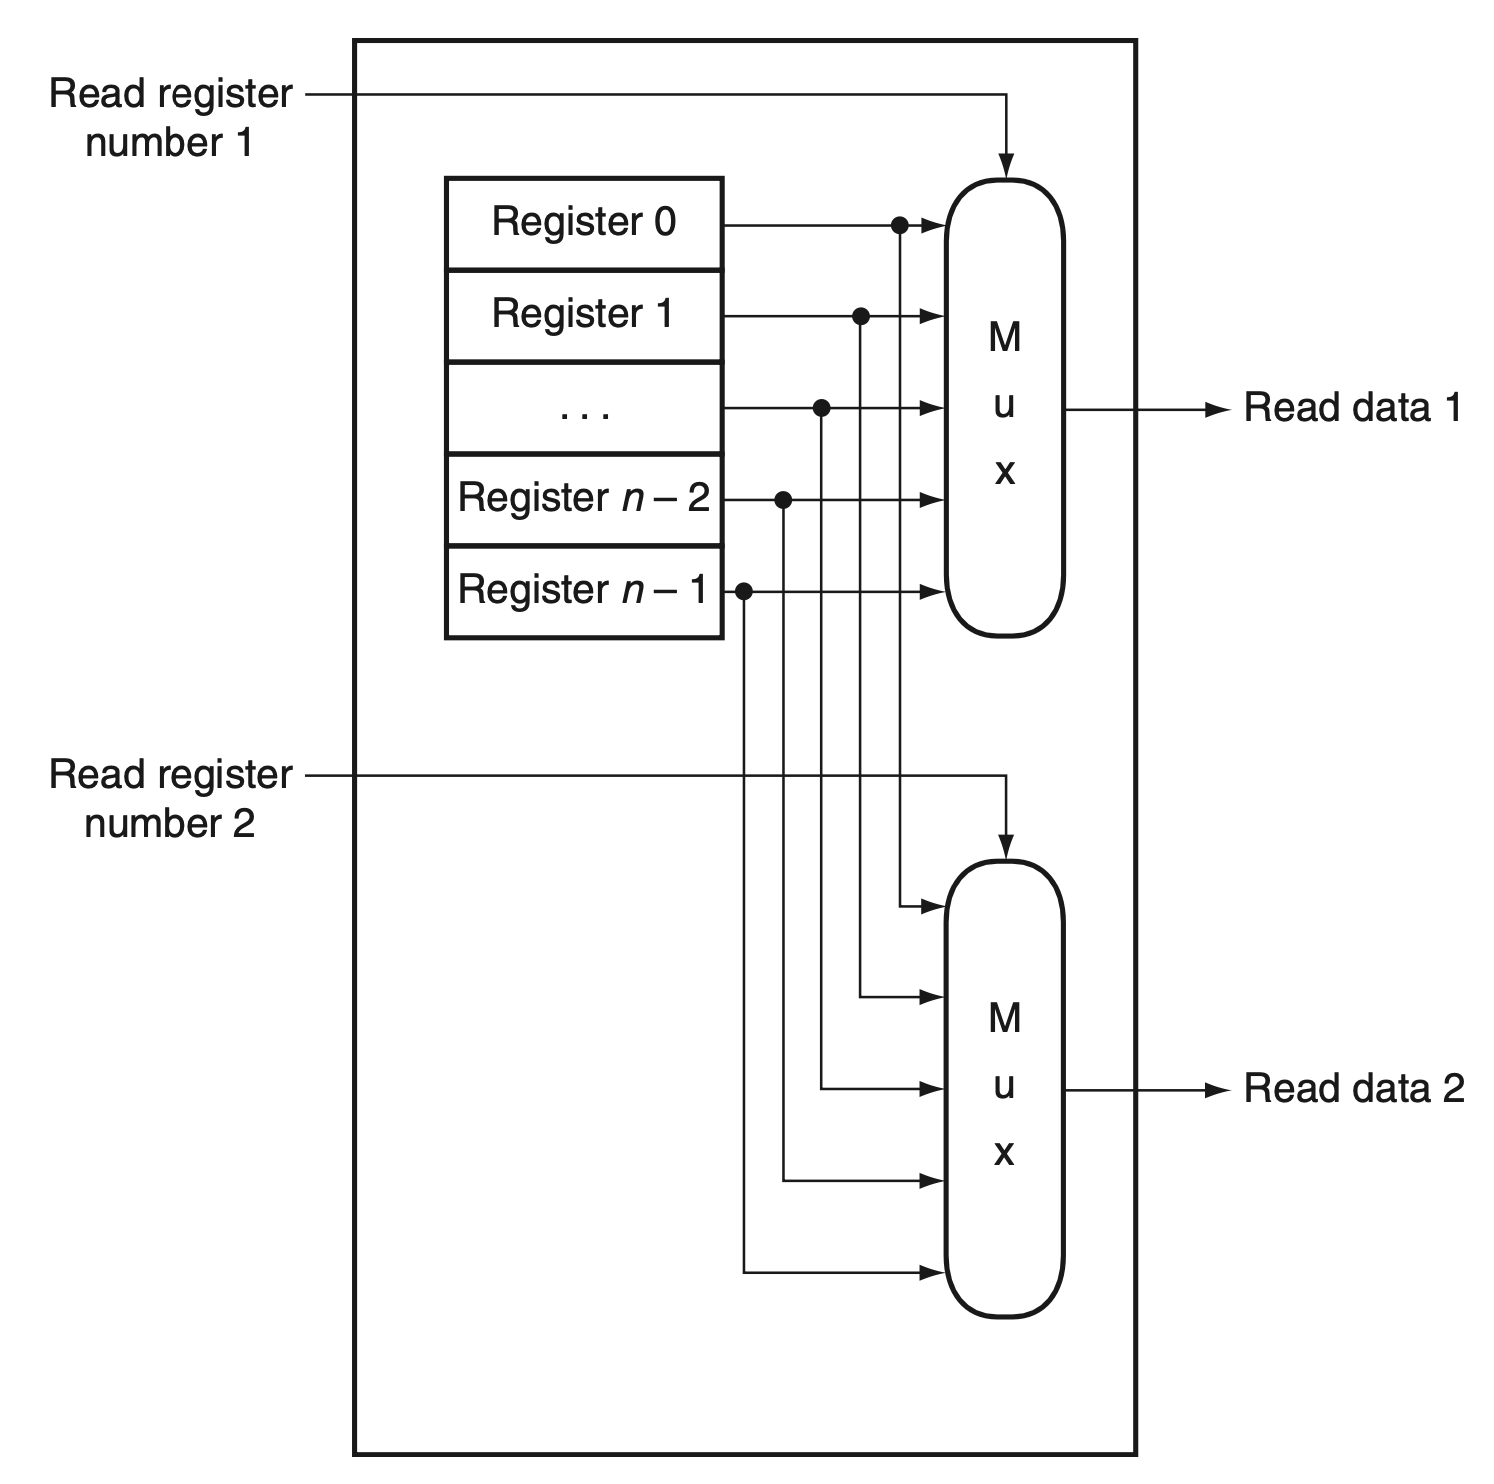
\includegraphics[width=0.55\linewidth]{img/regread1.png}
    }
    \caption{\textit{Read implementation in the register file}}
\end{figure}







% \begin{lstlisting}[caption={Simple SIGINT handler}]
% unsigned char stop = 0;
%
% void signal_handler(int x) {
%     stop = 1;
% }
%
% int main(void) {
%     signal(SIGINT, signal_handler);
%
%     /* Pressing Ctrl-C invokes signal_handler() */
%
%     while (!stop);
%     return 0;
% }
% \end{lstlisting}
%
% This is an example of an image.
%
% \begin{figure}[htbp]
%   \centering
%
%   \fcolorbox{codeFrame}{white}{%
%     \includegraphics[width=0.5\linewidth]{img/graph.png}%
%   }
%
%   \caption{My example image}
%   \label{fig:example}
% \end{figure}



\end{document}
